% Created by tikzDevice version 0.12.3.1 on 2021-07-04 23:19:06
% !TEX encoding = UTF-8 Unicode
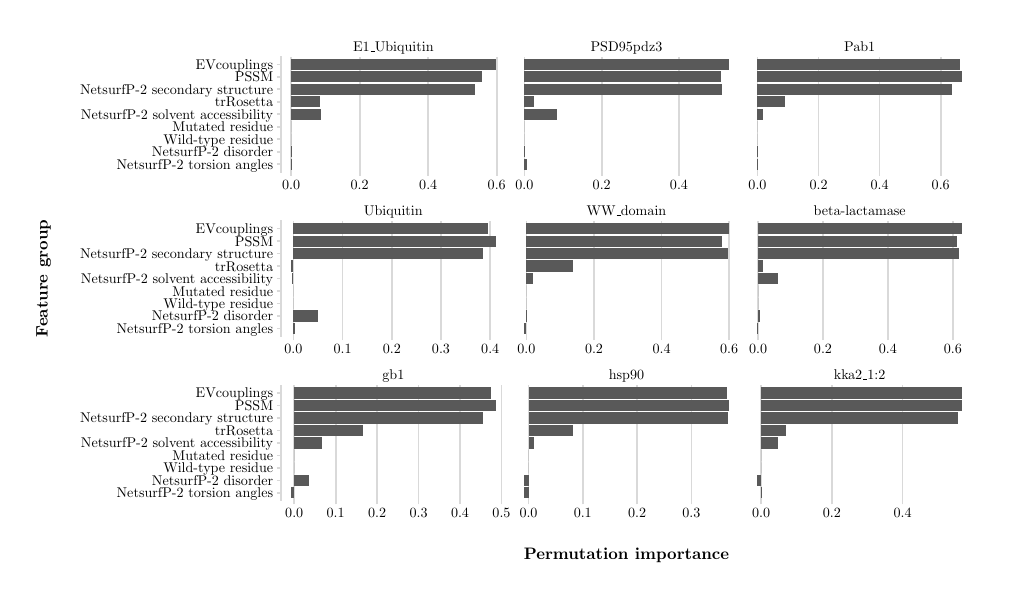
\begin{tikzpicture}[x=1pt,y=1pt]
\definecolor{fillColor}{RGB}{255,255,255}
\path[use as bounding box,fill=fillColor,fill opacity=0.00] (0,0) rectangle (344.26,196.49);
\begin{scope}
\path[clip] ( 91.51,144.44) rectangle (172.76,185.94);
\definecolor{drawColor}{gray}{0.85}

\path[draw=drawColor,line width= 0.6pt,line join=round] ( 95.21,144.44) --
	( 95.21,185.94);

\path[draw=drawColor,line width= 0.6pt,line join=round] (119.98,144.44) --
	(119.98,185.94);

\path[draw=drawColor,line width= 0.6pt,line join=round] (144.74,144.44) --
	(144.74,185.94);

\path[draw=drawColor,line width= 0.6pt,line join=round] (169.50,144.44) --
	(169.50,185.94);
\definecolor{fillColor}{gray}{0.35}

\path[fill=fillColor] ( 95.21,167.67) rectangle (105.68,171.73);

\path[fill=fillColor] ( 95.21,176.70) rectangle (164.15,180.76);

\path[fill=fillColor] ( 95.21,163.16) rectangle (106.15,167.22);

\path[fill=fillColor] ( 95.21,172.18) rectangle (161.69,176.24);

\path[fill=fillColor] ( 95.21,149.63) rectangle ( 95.22,153.69);

\path[fill=fillColor] ( 95.20,145.12) rectangle ( 95.21,149.18);

\path[fill=fillColor] ( 95.21,181.21) rectangle (169.06,185.27);

\path[fill=fillColor] ( 95.21,154.14) rectangle ( 95.21,158.20);

\path[fill=fillColor] ( 95.21,158.65) rectangle ( 95.21,162.71);
\end{scope}
\begin{scope}
\path[clip] ( 91.51, 85.06) rectangle (172.76,126.57);
\definecolor{drawColor}{gray}{0.85}

\path[draw=drawColor,line width= 0.6pt,line join=round] ( 96.01, 85.06) --
	( 96.01,126.57);

\path[draw=drawColor,line width= 0.6pt,line join=round] (113.79, 85.06) --
	(113.79,126.57);

\path[draw=drawColor,line width= 0.6pt,line join=round] (131.58, 85.06) --
	(131.58,126.57);

\path[draw=drawColor,line width= 0.6pt,line join=round] (149.36, 85.06) --
	(149.36,126.57);

\path[draw=drawColor,line width= 0.6pt,line join=round] (167.15, 85.06) --
	(167.15,126.57);
\definecolor{fillColor}{gray}{0.35}

\path[fill=fillColor] ( 95.20,108.30) rectangle ( 96.01,112.36);

\path[fill=fillColor] ( 96.01,117.32) rectangle (169.06,121.38);

\path[fill=fillColor] ( 95.52,103.79) rectangle ( 96.01,107.85);

\path[fill=fillColor] ( 96.01,112.81) rectangle (164.66,116.87);

\path[fill=fillColor] ( 96.01, 90.25) rectangle (104.84, 94.31);

\path[fill=fillColor] ( 96.01, 85.74) rectangle ( 96.42, 89.80);

\path[fill=fillColor] ( 96.01,121.83) rectangle (166.49,125.89);

\path[fill=fillColor] ( 96.01, 94.76) rectangle ( 96.01, 98.82);

\path[fill=fillColor] ( 96.01, 99.28) rectangle ( 96.01,103.34);
\end{scope}
\begin{scope}
\path[clip] ( 91.51, 25.69) rectangle (172.76, 67.19);
\definecolor{drawColor}{gray}{0.85}

\path[draw=drawColor,line width= 0.6pt,line join=round] ( 96.33, 25.69) --
	( 96.33, 67.19);

\path[draw=drawColor,line width= 0.6pt,line join=round] (111.30, 25.69) --
	(111.30, 67.19);

\path[draw=drawColor,line width= 0.6pt,line join=round] (126.28, 25.69) --
	(126.28, 67.19);

\path[draw=drawColor,line width= 0.6pt,line join=round] (141.26, 25.69) --
	(141.26, 67.19);

\path[draw=drawColor,line width= 0.6pt,line join=round] (156.23, 25.69) --
	(156.23, 67.19);

\path[draw=drawColor,line width= 0.6pt,line join=round] (171.21, 25.69) --
	(171.21, 67.19);
\definecolor{fillColor}{gray}{0.35}

\path[fill=fillColor] ( 96.33, 48.92) rectangle (121.07, 52.98);

\path[fill=fillColor] ( 96.33, 57.95) rectangle (169.06, 62.01);

\path[fill=fillColor] ( 96.33, 44.41) rectangle (106.28, 48.47);

\path[fill=fillColor] ( 96.33, 53.43) rectangle (164.43, 57.49);

\path[fill=fillColor] ( 96.33, 30.88) rectangle (101.79, 34.94);

\path[fill=fillColor] ( 95.20, 26.37) rectangle ( 96.33, 30.43);

\path[fill=fillColor] ( 96.33, 62.46) rectangle (167.53, 66.52);

\path[fill=fillColor] ( 96.33, 35.39) rectangle ( 96.33, 39.45);

\path[fill=fillColor] ( 96.33, 39.90) rectangle ( 96.33, 43.96);
\end{scope}
\begin{scope}
\path[clip] (175.76,144.44) rectangle (257.01,185.94);
\definecolor{drawColor}{gray}{0.85}

\path[draw=drawColor,line width= 0.6pt,line join=round] (179.50,144.44) --
	(179.50,185.94);

\path[draw=drawColor,line width= 0.6pt,line join=round] (207.43,144.44) --
	(207.43,185.94);

\path[draw=drawColor,line width= 0.6pt,line join=round] (235.36,144.44) --
	(235.36,185.94);
\definecolor{fillColor}{gray}{0.35}

\path[fill=fillColor] (179.50,167.67) rectangle (183.06,171.73);

\path[fill=fillColor] (179.50,176.70) rectangle (250.40,180.76);

\path[fill=fillColor] (179.50,163.16) rectangle (191.24,167.22);

\path[fill=fillColor] (179.50,172.18) rectangle (251.03,176.24);

\path[fill=fillColor] (179.45,149.63) rectangle (179.50,153.69);

\path[fill=fillColor] (179.50,145.12) rectangle (180.26,149.18);

\path[fill=fillColor] (179.50,181.21) rectangle (253.32,185.27);

\path[fill=fillColor] (179.50,154.14) rectangle (179.50,158.20);

\path[fill=fillColor] (179.50,158.65) rectangle (179.50,162.71);
\end{scope}
\begin{scope}
\path[clip] (175.76, 85.06) rectangle (257.01,126.57);
\definecolor{drawColor}{gray}{0.85}

\path[draw=drawColor,line width= 0.6pt,line join=round] (180.23, 85.06) --
	(180.23,126.57);

\path[draw=drawColor,line width= 0.6pt,line join=round] (204.65, 85.06) --
	(204.65,126.57);

\path[draw=drawColor,line width= 0.6pt,line join=round] (229.07, 85.06) --
	(229.07,126.57);

\path[draw=drawColor,line width= 0.6pt,line join=round] (253.49, 85.06) --
	(253.49,126.57);
\definecolor{fillColor}{gray}{0.35}

\path[fill=fillColor] (180.23,108.30) rectangle (197.22,112.36);

\path[fill=fillColor] (180.23,117.32) rectangle (250.98,121.38);

\path[fill=fillColor] (180.23,103.79) rectangle (182.50,107.85);

\path[fill=fillColor] (180.23,112.81) rectangle (253.09,116.87);

\path[fill=fillColor] (180.21, 90.25) rectangle (180.23, 94.31);

\path[fill=fillColor] (179.45, 85.74) rectangle (180.23, 89.80);

\path[fill=fillColor] (180.23,121.83) rectangle (253.32,125.89);

\path[fill=fillColor] (180.23, 94.76) rectangle (180.23, 98.82);

\path[fill=fillColor] (180.23, 99.28) rectangle (180.23,103.34);
\end{scope}
\begin{scope}
\path[clip] (175.76, 25.69) rectangle (257.01, 67.19);
\definecolor{drawColor}{gray}{0.85}

\path[draw=drawColor,line width= 0.6pt,line join=round] (180.98, 25.69) --
	(180.98, 67.19);

\path[draw=drawColor,line width= 0.6pt,line join=round] (200.59, 25.69) --
	(200.59, 67.19);

\path[draw=drawColor,line width= 0.6pt,line join=round] (220.20, 25.69) --
	(220.20, 67.19);

\path[draw=drawColor,line width= 0.6pt,line join=round] (239.81, 25.69) --
	(239.81, 67.19);
\definecolor{fillColor}{gray}{0.35}

\path[fill=fillColor] (180.98, 48.92) rectangle (197.13, 52.98);

\path[fill=fillColor] (180.98, 57.95) rectangle (253.32, 62.01);

\path[fill=fillColor] (180.98, 44.41) rectangle (182.93, 48.47);

\path[fill=fillColor] (180.98, 53.43) rectangle (253.17, 57.49);

\path[fill=fillColor] (179.45, 30.88) rectangle (180.98, 34.94);

\path[fill=fillColor] (179.52, 26.37) rectangle (180.98, 30.43);

\path[fill=fillColor] (180.98, 62.46) rectangle (252.70, 66.52);

\path[fill=fillColor] (180.98, 35.39) rectangle (180.98, 39.45);

\path[fill=fillColor] (180.98, 39.90) rectangle (180.98, 43.96);
\end{scope}
\begin{scope}
\path[clip] (260.01,144.44) rectangle (341.26,185.94);
\definecolor{drawColor}{gray}{0.85}

\path[draw=drawColor,line width= 0.6pt,line join=round] (263.71,144.44) --
	(263.71,185.94);

\path[draw=drawColor,line width= 0.6pt,line join=round] (285.79,144.44) --
	(285.79,185.94);

\path[draw=drawColor,line width= 0.6pt,line join=round] (307.86,144.44) --
	(307.86,185.94);

\path[draw=drawColor,line width= 0.6pt,line join=round] (329.93,144.44) --
	(329.93,185.94);
\definecolor{fillColor}{gray}{0.35}

\path[fill=fillColor] (263.71,167.67) rectangle (273.52,171.73);

\path[fill=fillColor] (263.71,176.70) rectangle (337.57,180.76);

\path[fill=fillColor] (263.71,163.16) rectangle (265.70,167.22);

\path[fill=fillColor] (263.71,172.18) rectangle (334.15,176.24);

\path[fill=fillColor] (263.70,149.63) rectangle (263.71,153.69);

\path[fill=fillColor] (263.71,145.12) rectangle (263.79,149.18);

\path[fill=fillColor] (263.71,181.21) rectangle (336.93,185.27);

\path[fill=fillColor] (263.71,154.14) rectangle (263.71,158.20);

\path[fill=fillColor] (263.71,158.65) rectangle (263.71,162.71);
\end{scope}
\begin{scope}
\path[clip] (260.01, 85.06) rectangle (341.26,126.57);
\definecolor{drawColor}{gray}{0.85}

\path[draw=drawColor,line width= 0.6pt,line join=round] (263.93, 85.06) --
	(263.93,126.57);

\path[draw=drawColor,line width= 0.6pt,line join=round] (287.39, 85.06) --
	(287.39,126.57);

\path[draw=drawColor,line width= 0.6pt,line join=round] (310.85, 85.06) --
	(310.85,126.57);

\path[draw=drawColor,line width= 0.6pt,line join=round] (334.31, 85.06) --
	(334.31,126.57);
\definecolor{fillColor}{gray}{0.35}

\path[fill=fillColor] (263.93,108.30) rectangle (265.56,112.36);

\path[fill=fillColor] (263.93,117.32) rectangle (335.77,121.38);

\path[fill=fillColor] (263.93,103.79) rectangle (271.30,107.85);

\path[fill=fillColor] (263.93,112.81) rectangle (336.38,116.87);

\path[fill=fillColor] (263.93, 90.25) rectangle (264.78, 94.31);

\path[fill=fillColor] (263.70, 85.74) rectangle (263.93, 89.80);

\path[fill=fillColor] (263.93,121.83) rectangle (337.57,125.89);

\path[fill=fillColor] (263.93, 94.76) rectangle (263.93, 98.82);

\path[fill=fillColor] (263.93, 99.28) rectangle (263.93,103.34);
\end{scope}
\begin{scope}
\path[clip] (260.01, 25.69) rectangle (341.26, 67.19);
\definecolor{drawColor}{gray}{0.85}

\path[draw=drawColor,line width= 0.6pt,line join=round] (265.01, 25.69) --
	(265.01, 67.19);

\path[draw=drawColor,line width= 0.6pt,line join=round] (290.58, 25.69) --
	(290.58, 67.19);

\path[draw=drawColor,line width= 0.6pt,line join=round] (316.16, 25.69) --
	(316.16, 67.19);
\definecolor{fillColor}{gray}{0.35}

\path[fill=fillColor] (265.01, 48.92) rectangle (274.11, 52.98);

\path[fill=fillColor] (265.01, 57.95) rectangle (337.44, 62.01);

\path[fill=fillColor] (265.01, 44.41) rectangle (271.24, 48.47);

\path[fill=fillColor] (265.01, 53.43) rectangle (336.02, 57.49);

\path[fill=fillColor] (263.70, 30.88) rectangle (265.01, 34.94);

\path[fill=fillColor] (265.01, 26.37) rectangle (265.12, 30.43);

\path[fill=fillColor] (265.01, 62.46) rectangle (337.57, 66.52);

\path[fill=fillColor] (265.01, 35.39) rectangle (265.01, 39.45);

\path[fill=fillColor] (265.01, 39.90) rectangle (265.01, 43.96);
\end{scope}
\begin{scope}
\path[clip] ( 91.51, 67.19) rectangle (172.76, 74.74);
\definecolor{drawColor}{RGB}{0,0,0}

\node[text=drawColor,anchor=base,inner sep=0pt, outer sep=0pt, scale=  0.51] at (132.13, 69.19) {gb1};
\end{scope}
\begin{scope}
\path[clip] (175.76, 67.19) rectangle (257.01, 74.74);
\definecolor{drawColor}{RGB}{0,0,0}

\node[text=drawColor,anchor=base,inner sep=0pt, outer sep=0pt, scale=  0.51] at (216.38, 69.19) {hsp90};
\end{scope}
\begin{scope}
\path[clip] (260.01, 67.19) rectangle (341.26, 74.74);
\definecolor{drawColor}{RGB}{0,0,0}

\node[text=drawColor,anchor=base,inner sep=0pt, outer sep=0pt, scale=  0.51] at (300.64, 69.19) {kka2\_1:2};
\end{scope}
\begin{scope}
\path[clip] ( 91.51,126.57) rectangle (172.76,134.11);
\definecolor{drawColor}{RGB}{0,0,0}

\node[text=drawColor,anchor=base,inner sep=0pt, outer sep=0pt, scale=  0.51] at (132.13,128.57) {Ubiquitin};
\end{scope}
\begin{scope}
\path[clip] (175.76,126.57) rectangle (257.01,134.11);
\definecolor{drawColor}{RGB}{0,0,0}

\node[text=drawColor,anchor=base,inner sep=0pt, outer sep=0pt, scale=  0.51] at (216.38,128.57) {WW\_domain};
\end{scope}
\begin{scope}
\path[clip] (260.01,126.57) rectangle (341.26,134.11);
\definecolor{drawColor}{RGB}{0,0,0}

\node[text=drawColor,anchor=base,inner sep=0pt, outer sep=0pt, scale=  0.51] at (300.64,128.57) {beta-lactamase};
\end{scope}
\begin{scope}
\path[clip] ( 91.51,185.94) rectangle (172.76,193.49);
\definecolor{drawColor}{RGB}{0,0,0}

\node[text=drawColor,anchor=base,inner sep=0pt, outer sep=0pt, scale=  0.51] at (132.13,187.94) {E1\_Ubiquitin};
\end{scope}
\begin{scope}
\path[clip] (175.76,185.94) rectangle (257.01,193.49);
\definecolor{drawColor}{RGB}{0,0,0}

\node[text=drawColor,anchor=base,inner sep=0pt, outer sep=0pt, scale=  0.51] at (216.38,187.94) {PSD95pdz3};
\end{scope}
\begin{scope}
\path[clip] (260.01,185.94) rectangle (341.26,193.49);
\definecolor{drawColor}{RGB}{0,0,0}

\node[text=drawColor,anchor=base,inner sep=0pt, outer sep=0pt, scale=  0.51] at (300.64,187.94) {Pab1};
\end{scope}
\begin{scope}
\path[clip] (  0.00,  0.00) rectangle (344.26,196.49);
\definecolor{drawColor}{gray}{0.85}

\path[draw=drawColor,line width= 0.6pt,line join=round] ( 96.33, 24.19) --
	( 96.33, 25.69);

\path[draw=drawColor,line width= 0.6pt,line join=round] (111.30, 24.19) --
	(111.30, 25.69);

\path[draw=drawColor,line width= 0.6pt,line join=round] (126.28, 24.19) --
	(126.28, 25.69);

\path[draw=drawColor,line width= 0.6pt,line join=round] (141.26, 24.19) --
	(141.26, 25.69);

\path[draw=drawColor,line width= 0.6pt,line join=round] (156.23, 24.19) --
	(156.23, 25.69);

\path[draw=drawColor,line width= 0.6pt,line join=round] (171.21, 24.19) --
	(171.21, 25.69);
\end{scope}
\begin{scope}
\path[clip] (  0.00,  0.00) rectangle (344.26,196.49);
\definecolor{drawColor}{RGB}{0,0,0}

\node[text=drawColor,anchor=base,inner sep=0pt, outer sep=0pt, scale=  0.51] at ( 96.33, 19.36) {0.0};

\node[text=drawColor,anchor=base,inner sep=0pt, outer sep=0pt, scale=  0.51] at (111.30, 19.36) {0.1};

\node[text=drawColor,anchor=base,inner sep=0pt, outer sep=0pt, scale=  0.51] at (126.28, 19.36) {0.2};

\node[text=drawColor,anchor=base,inner sep=0pt, outer sep=0pt, scale=  0.51] at (141.26, 19.36) {0.3};

\node[text=drawColor,anchor=base,inner sep=0pt, outer sep=0pt, scale=  0.51] at (156.23, 19.36) {0.4};

\node[text=drawColor,anchor=base,inner sep=0pt, outer sep=0pt, scale=  0.51] at (171.21, 19.36) {0.5};
\end{scope}
\begin{scope}
\path[clip] (  0.00,  0.00) rectangle (344.26,196.49);
\definecolor{drawColor}{gray}{0.85}

\path[draw=drawColor,line width= 0.6pt,line join=round] (180.98, 24.19) --
	(180.98, 25.69);

\path[draw=drawColor,line width= 0.6pt,line join=round] (200.59, 24.19) --
	(200.59, 25.69);

\path[draw=drawColor,line width= 0.6pt,line join=round] (220.20, 24.19) --
	(220.20, 25.69);

\path[draw=drawColor,line width= 0.6pt,line join=round] (239.81, 24.19) --
	(239.81, 25.69);
\end{scope}
\begin{scope}
\path[clip] (  0.00,  0.00) rectangle (344.26,196.49);
\definecolor{drawColor}{RGB}{0,0,0}

\node[text=drawColor,anchor=base,inner sep=0pt, outer sep=0pt, scale=  0.51] at (180.98, 19.36) {0.0};

\node[text=drawColor,anchor=base,inner sep=0pt, outer sep=0pt, scale=  0.51] at (200.59, 19.36) {0.1};

\node[text=drawColor,anchor=base,inner sep=0pt, outer sep=0pt, scale=  0.51] at (220.20, 19.36) {0.2};

\node[text=drawColor,anchor=base,inner sep=0pt, outer sep=0pt, scale=  0.51] at (239.81, 19.36) {0.3};
\end{scope}
\begin{scope}
\path[clip] (  0.00,  0.00) rectangle (344.26,196.49);
\definecolor{drawColor}{gray}{0.85}

\path[draw=drawColor,line width= 0.6pt,line join=round] (265.01, 24.19) --
	(265.01, 25.69);

\path[draw=drawColor,line width= 0.6pt,line join=round] (290.58, 24.19) --
	(290.58, 25.69);

\path[draw=drawColor,line width= 0.6pt,line join=round] (316.16, 24.19) --
	(316.16, 25.69);
\end{scope}
\begin{scope}
\path[clip] (  0.00,  0.00) rectangle (344.26,196.49);
\definecolor{drawColor}{RGB}{0,0,0}

\node[text=drawColor,anchor=base,inner sep=0pt, outer sep=0pt, scale=  0.51] at (265.01, 19.36) {0.0};

\node[text=drawColor,anchor=base,inner sep=0pt, outer sep=0pt, scale=  0.51] at (290.58, 19.36) {0.2};

\node[text=drawColor,anchor=base,inner sep=0pt, outer sep=0pt, scale=  0.51] at (316.16, 19.36) {0.4};
\end{scope}
\begin{scope}
\path[clip] (  0.00,  0.00) rectangle (344.26,196.49);
\definecolor{drawColor}{gray}{0.85}

\path[draw=drawColor,line width= 0.6pt,line join=round] ( 96.01, 83.56) --
	( 96.01, 85.06);

\path[draw=drawColor,line width= 0.6pt,line join=round] (113.79, 83.56) --
	(113.79, 85.06);

\path[draw=drawColor,line width= 0.6pt,line join=round] (131.58, 83.56) --
	(131.58, 85.06);

\path[draw=drawColor,line width= 0.6pt,line join=round] (149.36, 83.56) --
	(149.36, 85.06);

\path[draw=drawColor,line width= 0.6pt,line join=round] (167.15, 83.56) --
	(167.15, 85.06);
\end{scope}
\begin{scope}
\path[clip] (  0.00,  0.00) rectangle (344.26,196.49);
\definecolor{drawColor}{RGB}{0,0,0}

\node[text=drawColor,anchor=base,inner sep=0pt, outer sep=0pt, scale=  0.51] at ( 96.01, 78.74) {0.0};

\node[text=drawColor,anchor=base,inner sep=0pt, outer sep=0pt, scale=  0.51] at (113.79, 78.74) {0.1};

\node[text=drawColor,anchor=base,inner sep=0pt, outer sep=0pt, scale=  0.51] at (131.58, 78.74) {0.2};

\node[text=drawColor,anchor=base,inner sep=0pt, outer sep=0pt, scale=  0.51] at (149.36, 78.74) {0.3};

\node[text=drawColor,anchor=base,inner sep=0pt, outer sep=0pt, scale=  0.51] at (167.15, 78.74) {0.4};
\end{scope}
\begin{scope}
\path[clip] (  0.00,  0.00) rectangle (344.26,196.49);
\definecolor{drawColor}{gray}{0.85}

\path[draw=drawColor,line width= 0.6pt,line join=round] (180.23, 83.56) --
	(180.23, 85.06);

\path[draw=drawColor,line width= 0.6pt,line join=round] (204.65, 83.56) --
	(204.65, 85.06);

\path[draw=drawColor,line width= 0.6pt,line join=round] (229.07, 83.56) --
	(229.07, 85.06);

\path[draw=drawColor,line width= 0.6pt,line join=round] (253.49, 83.56) --
	(253.49, 85.06);
\end{scope}
\begin{scope}
\path[clip] (  0.00,  0.00) rectangle (344.26,196.49);
\definecolor{drawColor}{RGB}{0,0,0}

\node[text=drawColor,anchor=base,inner sep=0pt, outer sep=0pt, scale=  0.51] at (180.23, 78.74) {0.0};

\node[text=drawColor,anchor=base,inner sep=0pt, outer sep=0pt, scale=  0.51] at (204.65, 78.74) {0.2};

\node[text=drawColor,anchor=base,inner sep=0pt, outer sep=0pt, scale=  0.51] at (229.07, 78.74) {0.4};

\node[text=drawColor,anchor=base,inner sep=0pt, outer sep=0pt, scale=  0.51] at (253.49, 78.74) {0.6};
\end{scope}
\begin{scope}
\path[clip] (  0.00,  0.00) rectangle (344.26,196.49);
\definecolor{drawColor}{gray}{0.85}

\path[draw=drawColor,line width= 0.6pt,line join=round] (263.93, 83.56) --
	(263.93, 85.06);

\path[draw=drawColor,line width= 0.6pt,line join=round] (287.39, 83.56) --
	(287.39, 85.06);

\path[draw=drawColor,line width= 0.6pt,line join=round] (310.85, 83.56) --
	(310.85, 85.06);

\path[draw=drawColor,line width= 0.6pt,line join=round] (334.31, 83.56) --
	(334.31, 85.06);
\end{scope}
\begin{scope}
\path[clip] (  0.00,  0.00) rectangle (344.26,196.49);
\definecolor{drawColor}{RGB}{0,0,0}

\node[text=drawColor,anchor=base,inner sep=0pt, outer sep=0pt, scale=  0.51] at (263.93, 78.74) {0.0};

\node[text=drawColor,anchor=base,inner sep=0pt, outer sep=0pt, scale=  0.51] at (287.39, 78.74) {0.2};

\node[text=drawColor,anchor=base,inner sep=0pt, outer sep=0pt, scale=  0.51] at (310.85, 78.74) {0.4};

\node[text=drawColor,anchor=base,inner sep=0pt, outer sep=0pt, scale=  0.51] at (334.31, 78.74) {0.6};
\end{scope}
\begin{scope}
\path[clip] (  0.00,  0.00) rectangle (344.26,196.49);
\definecolor{drawColor}{gray}{0.85}

\path[draw=drawColor,line width= 0.6pt,line join=round] ( 95.21,142.94) --
	( 95.21,144.44);

\path[draw=drawColor,line width= 0.6pt,line join=round] (119.98,142.94) --
	(119.98,144.44);

\path[draw=drawColor,line width= 0.6pt,line join=round] (144.74,142.94) --
	(144.74,144.44);

\path[draw=drawColor,line width= 0.6pt,line join=round] (169.50,142.94) --
	(169.50,144.44);
\end{scope}
\begin{scope}
\path[clip] (  0.00,  0.00) rectangle (344.26,196.49);
\definecolor{drawColor}{RGB}{0,0,0}

\node[text=drawColor,anchor=base,inner sep=0pt, outer sep=0pt, scale=  0.51] at ( 95.21,138.11) {0.0};

\node[text=drawColor,anchor=base,inner sep=0pt, outer sep=0pt, scale=  0.51] at (119.98,138.11) {0.2};

\node[text=drawColor,anchor=base,inner sep=0pt, outer sep=0pt, scale=  0.51] at (144.74,138.11) {0.4};

\node[text=drawColor,anchor=base,inner sep=0pt, outer sep=0pt, scale=  0.51] at (169.50,138.11) {0.6};
\end{scope}
\begin{scope}
\path[clip] (  0.00,  0.00) rectangle (344.26,196.49);
\definecolor{drawColor}{gray}{0.85}

\path[draw=drawColor,line width= 0.6pt,line join=round] (179.50,142.94) --
	(179.50,144.44);

\path[draw=drawColor,line width= 0.6pt,line join=round] (207.43,142.94) --
	(207.43,144.44);

\path[draw=drawColor,line width= 0.6pt,line join=round] (235.36,142.94) --
	(235.36,144.44);
\end{scope}
\begin{scope}
\path[clip] (  0.00,  0.00) rectangle (344.26,196.49);
\definecolor{drawColor}{RGB}{0,0,0}

\node[text=drawColor,anchor=base,inner sep=0pt, outer sep=0pt, scale=  0.51] at (179.50,138.11) {0.0};

\node[text=drawColor,anchor=base,inner sep=0pt, outer sep=0pt, scale=  0.51] at (207.43,138.11) {0.2};

\node[text=drawColor,anchor=base,inner sep=0pt, outer sep=0pt, scale=  0.51] at (235.36,138.11) {0.4};
\end{scope}
\begin{scope}
\path[clip] (  0.00,  0.00) rectangle (344.26,196.49);
\definecolor{drawColor}{gray}{0.85}

\path[draw=drawColor,line width= 0.6pt,line join=round] (263.71,142.94) --
	(263.71,144.44);

\path[draw=drawColor,line width= 0.6pt,line join=round] (285.79,142.94) --
	(285.79,144.44);

\path[draw=drawColor,line width= 0.6pt,line join=round] (307.86,142.94) --
	(307.86,144.44);

\path[draw=drawColor,line width= 0.6pt,line join=round] (329.93,142.94) --
	(329.93,144.44);
\end{scope}
\begin{scope}
\path[clip] (  0.00,  0.00) rectangle (344.26,196.49);
\definecolor{drawColor}{RGB}{0,0,0}

\node[text=drawColor,anchor=base,inner sep=0pt, outer sep=0pt, scale=  0.51] at (263.71,138.11) {0.0};

\node[text=drawColor,anchor=base,inner sep=0pt, outer sep=0pt, scale=  0.51] at (285.79,138.11) {0.2};

\node[text=drawColor,anchor=base,inner sep=0pt, outer sep=0pt, scale=  0.51] at (307.86,138.11) {0.4};

\node[text=drawColor,anchor=base,inner sep=0pt, outer sep=0pt, scale=  0.51] at (329.93,138.11) {0.6};
\end{scope}
\begin{scope}
\path[clip] (  0.00,  0.00) rectangle (344.26,196.49);
\definecolor{drawColor}{gray}{0.85}

\path[draw=drawColor,line width= 0.6pt,line join=round,line cap=rect] ( 91.51,144.44) --
	( 91.51,185.94);
\end{scope}
\begin{scope}
\path[clip] (  0.00,  0.00) rectangle (344.26,196.49);
\definecolor{drawColor}{RGB}{0,0,0}

\node[text=drawColor,anchor=base east,inner sep=0pt, outer sep=0pt, scale=  0.51] at ( 88.72,145.38) {NetsurfP-2 torsion angles};

\node[text=drawColor,anchor=base east,inner sep=0pt, outer sep=0pt, scale=  0.51] at ( 88.72,149.89) {NetsurfP-2 disorder};

\node[text=drawColor,anchor=base east,inner sep=0pt, outer sep=0pt, scale=  0.51] at ( 88.72,154.40) {Wild-type residue};

\node[text=drawColor,anchor=base east,inner sep=0pt, outer sep=0pt, scale=  0.51] at ( 88.72,158.91) {Mutated residue};

\node[text=drawColor,anchor=base east,inner sep=0pt, outer sep=0pt, scale=  0.51] at ( 88.72,163.42) {NetsurfP-2 solvent accessibility};

\node[text=drawColor,anchor=base east,inner sep=0pt, outer sep=0pt, scale=  0.51] at ( 88.72,167.93) {trRosetta};

\node[text=drawColor,anchor=base east,inner sep=0pt, outer sep=0pt, scale=  0.51] at ( 88.72,172.44) {NetsurfP-2 secondary structure};

\node[text=drawColor,anchor=base east,inner sep=0pt, outer sep=0pt, scale=  0.51] at ( 88.72,176.95) {PSSM};

\node[text=drawColor,anchor=base east,inner sep=0pt, outer sep=0pt, scale=  0.51] at ( 88.72,181.47) {EVcouplings};
\end{scope}
\begin{scope}
\path[clip] (  0.00,  0.00) rectangle (344.26,196.49);
\definecolor{drawColor}{gray}{0.85}

\path[draw=drawColor,line width= 0.6pt,line join=round] ( 90.01,147.15) --
	( 91.51,147.15);

\path[draw=drawColor,line width= 0.6pt,line join=round] ( 90.01,151.66) --
	( 91.51,151.66);

\path[draw=drawColor,line width= 0.6pt,line join=round] ( 90.01,156.17) --
	( 91.51,156.17);

\path[draw=drawColor,line width= 0.6pt,line join=round] ( 90.01,160.68) --
	( 91.51,160.68);

\path[draw=drawColor,line width= 0.6pt,line join=round] ( 90.01,165.19) --
	( 91.51,165.19);

\path[draw=drawColor,line width= 0.6pt,line join=round] ( 90.01,169.70) --
	( 91.51,169.70);

\path[draw=drawColor,line width= 0.6pt,line join=round] ( 90.01,174.21) --
	( 91.51,174.21);

\path[draw=drawColor,line width= 0.6pt,line join=round] ( 90.01,178.73) --
	( 91.51,178.73);

\path[draw=drawColor,line width= 0.6pt,line join=round] ( 90.01,183.24) --
	( 91.51,183.24);
\end{scope}
\begin{scope}
\path[clip] (  0.00,  0.00) rectangle (344.26,196.49);
\definecolor{drawColor}{gray}{0.85}

\path[draw=drawColor,line width= 0.6pt,line join=round,line cap=rect] ( 91.51, 85.06) --
	( 91.51,126.57);
\end{scope}
\begin{scope}
\path[clip] (  0.00,  0.00) rectangle (344.26,196.49);
\definecolor{drawColor}{RGB}{0,0,0}

\node[text=drawColor,anchor=base east,inner sep=0pt, outer sep=0pt, scale=  0.51] at ( 88.72, 86.00) {NetsurfP-2 torsion angles};

\node[text=drawColor,anchor=base east,inner sep=0pt, outer sep=0pt, scale=  0.51] at ( 88.72, 90.51) {NetsurfP-2 disorder};

\node[text=drawColor,anchor=base east,inner sep=0pt, outer sep=0pt, scale=  0.51] at ( 88.72, 95.02) {Wild-type residue};

\node[text=drawColor,anchor=base east,inner sep=0pt, outer sep=0pt, scale=  0.51] at ( 88.72, 99.53) {Mutated residue};

\node[text=drawColor,anchor=base east,inner sep=0pt, outer sep=0pt, scale=  0.51] at ( 88.72,104.05) {NetsurfP-2 solvent accessibility};

\node[text=drawColor,anchor=base east,inner sep=0pt, outer sep=0pt, scale=  0.51] at ( 88.72,108.56) {trRosetta};

\node[text=drawColor,anchor=base east,inner sep=0pt, outer sep=0pt, scale=  0.51] at ( 88.72,113.07) {NetsurfP-2 secondary structure};

\node[text=drawColor,anchor=base east,inner sep=0pt, outer sep=0pt, scale=  0.51] at ( 88.72,117.58) {PSSM};

\node[text=drawColor,anchor=base east,inner sep=0pt, outer sep=0pt, scale=  0.51] at ( 88.72,122.09) {EVcouplings};
\end{scope}
\begin{scope}
\path[clip] (  0.00,  0.00) rectangle (344.26,196.49);
\definecolor{drawColor}{gray}{0.85}

\path[draw=drawColor,line width= 0.6pt,line join=round] ( 90.01, 87.77) --
	( 91.51, 87.77);

\path[draw=drawColor,line width= 0.6pt,line join=round] ( 90.01, 92.28) --
	( 91.51, 92.28);

\path[draw=drawColor,line width= 0.6pt,line join=round] ( 90.01, 96.79) --
	( 91.51, 96.79);

\path[draw=drawColor,line width= 0.6pt,line join=round] ( 90.01,101.31) --
	( 91.51,101.31);

\path[draw=drawColor,line width= 0.6pt,line join=round] ( 90.01,105.82) --
	( 91.51,105.82);

\path[draw=drawColor,line width= 0.6pt,line join=round] ( 90.01,110.33) --
	( 91.51,110.33);

\path[draw=drawColor,line width= 0.6pt,line join=round] ( 90.01,114.84) --
	( 91.51,114.84);

\path[draw=drawColor,line width= 0.6pt,line join=round] ( 90.01,119.35) --
	( 91.51,119.35);

\path[draw=drawColor,line width= 0.6pt,line join=round] ( 90.01,123.86) --
	( 91.51,123.86);
\end{scope}
\begin{scope}
\path[clip] (  0.00,  0.00) rectangle (344.26,196.49);
\definecolor{drawColor}{gray}{0.85}

\path[draw=drawColor,line width= 0.6pt,line join=round,line cap=rect] ( 91.51, 25.69) --
	( 91.51, 67.19);
\end{scope}
\begin{scope}
\path[clip] (  0.00,  0.00) rectangle (344.26,196.49);
\definecolor{drawColor}{RGB}{0,0,0}

\node[text=drawColor,anchor=base east,inner sep=0pt, outer sep=0pt, scale=  0.51] at ( 88.72, 26.62) {NetsurfP-2 torsion angles};

\node[text=drawColor,anchor=base east,inner sep=0pt, outer sep=0pt, scale=  0.51] at ( 88.72, 31.14) {NetsurfP-2 disorder};

\node[text=drawColor,anchor=base east,inner sep=0pt, outer sep=0pt, scale=  0.51] at ( 88.72, 35.65) {Wild-type residue};

\node[text=drawColor,anchor=base east,inner sep=0pt, outer sep=0pt, scale=  0.51] at ( 88.72, 40.16) {Mutated residue};

\node[text=drawColor,anchor=base east,inner sep=0pt, outer sep=0pt, scale=  0.51] at ( 88.72, 44.67) {NetsurfP-2 solvent accessibility};

\node[text=drawColor,anchor=base east,inner sep=0pt, outer sep=0pt, scale=  0.51] at ( 88.72, 49.18) {trRosetta};

\node[text=drawColor,anchor=base east,inner sep=0pt, outer sep=0pt, scale=  0.51] at ( 88.72, 53.69) {NetsurfP-2 secondary structure};

\node[text=drawColor,anchor=base east,inner sep=0pt, outer sep=0pt, scale=  0.51] at ( 88.72, 58.20) {PSSM};

\node[text=drawColor,anchor=base east,inner sep=0pt, outer sep=0pt, scale=  0.51] at ( 88.72, 62.72) {EVcouplings};
\end{scope}
\begin{scope}
\path[clip] (  0.00,  0.00) rectangle (344.26,196.49);
\definecolor{drawColor}{gray}{0.85}

\path[draw=drawColor,line width= 0.6pt,line join=round] ( 90.01, 28.40) --
	( 91.51, 28.40);

\path[draw=drawColor,line width= 0.6pt,line join=round] ( 90.01, 32.91) --
	( 91.51, 32.91);

\path[draw=drawColor,line width= 0.6pt,line join=round] ( 90.01, 37.42) --
	( 91.51, 37.42);

\path[draw=drawColor,line width= 0.6pt,line join=round] ( 90.01, 41.93) --
	( 91.51, 41.93);

\path[draw=drawColor,line width= 0.6pt,line join=round] ( 90.01, 46.44) --
	( 91.51, 46.44);

\path[draw=drawColor,line width= 0.6pt,line join=round] ( 90.01, 50.95) --
	( 91.51, 50.95);

\path[draw=drawColor,line width= 0.6pt,line join=round] ( 90.01, 55.46) --
	( 91.51, 55.46);

\path[draw=drawColor,line width= 0.6pt,line join=round] ( 90.01, 59.98) --
	( 91.51, 59.98);

\path[draw=drawColor,line width= 0.6pt,line join=round] ( 90.01, 64.49) --
	( 91.51, 64.49);
\end{scope}
\begin{scope}
\path[clip] (  0.00,  0.00) rectangle (344.26,196.49);
\definecolor{drawColor}{RGB}{0,0,0}

\node[text=drawColor,anchor=base,inner sep=0pt, outer sep=0pt, scale=  0.60] at (216.38,  4.17) {\bfseries Permutation importance};
\end{scope}
\begin{scope}
\path[clip] (  0.00,  0.00) rectangle (344.26,196.49);
\definecolor{drawColor}{RGB}{0,0,0}

\node[text=drawColor,rotate= 90.00,anchor=base,inner sep=0pt, outer sep=0pt, scale=  0.60] at (  7.19,105.82) {\bfseries Feature group};
\end{scope}
\end{tikzpicture}%
